% Copyright 2004 by Till Tantau <tantau@users.sourceforge.net>.
%
% In principle, this file can be redistributed and/or modified under
% the terms of the GNU Public License, version 2.
%
% However, this file is supposed to be a template to be modified
% for your own needs. For this reason, if you use this file as a
% template and not specifically distribute it as part of a another
% package/program, I grant the extra permission to freely copy and
% modify this file as you see fit and even to delete this copyright
% notice. 

\documentclass{beamer}
% Replace the \documentclass declaration above
% with the following two lines to typeset your 
% lecture notes as a handout:
%\documentclass{article}
%\usepackage{beamerarticle}


% There are many different themes available for Beamer. A comprehensive
% list with examples is given here:
% http://deic.uab.es/~iblanes/beamer_gallery/index_by_theme.html
% You can uncomment the themes below if you would like to use a different
% one:
%\usetheme{AnnArbor}
%\usetheme{Antibes}
%\usetheme{Bergen}
%\usetheme{Berkeley}
%\usetheme{Berlin}
%\usetheme{Boadilla}
%\usetheme{boxes}
\usetheme{CambridgeUS} %:3
%\usetheme{Copenhagen}
%\usetheme{Darmstadt}
%\usetheme{default}
%\usetheme{Frankfurt}
%\usetheme{Goettingen}
%\usetheme{Hannover}
%\usetheme{Ilmenau}
%\usetheme{JuanLesPins}
%\usetheme{Luebeck}
%\usetheme{Madrid}
%\usetheme{Malmoe}
%\usetheme{Marburg}
%\usetheme{Montpellier}
%\usetheme{PaloAlto}
%\usetheme{Pittsburgh}
%\usetheme{Rochester}
%\usetheme{Singapore}
%\usetheme{Szeged}
%\usetheme{Warsaw}

\usepackage{answers}
\usepackage{setspace}
\usepackage{graphicx}
\usepackage{enumerate}
\usepackage{multicol}
\usepackage{mathrsfs}
\usepackage[spanish]{babel}
\usepackage[utf8]{inputenc}
\usepackage{tikz}
\usepackage{verbatim} 
\definecolor{gey}{rgb}{0.8, 0.8, 0.8}

\newcommand{\N}{\mathbb{N}}
\newcommand{\Z}{\mathbb{Z}}
\newcommand{\C}{\mathbb{C}}
\newcommand{\R}{\mathbb{R}}


\title{EDP}

% A subtitle is optional and this may be deleted
\subtitle{Optional Subtitle}

\author{Miguel, Diana }
% - Give the names in the same order as the appear in the paper.
% - Use the \inst{?} command only if the authors have different
%   affiliation.

\institute[Konrad Lorenz] % (optional, but mostly needed)
{
  \inst{1}%
  Department of Computer Science\\
  University of Somewhere
  \and
  \inst{2}%
  Department of Theoretical Philosophy\\
  University of Elsewhere}
% - Use the \inst command only if there are several affiliations.
% - Keep it simple, no one is interested in your street address.

\date{}
% - Either use conference name or its abbreviation.
% - Not really informative to the audience, more for people (including
%   yourself) who are reading the slides online

\subject{Theoretical Computer Science}
% This is only inserted into the PDF information catalog. Can be left
% out. 

% If you have a file called "university-logo-filename.xxx", where xxx
% is a graphic format that can be processed by latex or pdflatex,
% resp., then you can add a logo as follows:

% \pgfdeclareimage[height=0.5cm]{university-logo}{university-logo-filename}
% \logo{\pgfuseimage{university-logo}}

% Delete this, if you do not want the table of contents to pop up at
% the beginning of each subsection:
\AtBeginSubsection[]
{
  \begin{frame}<beamer>{Outline}
    \tableofcontents[currentsection,currentsubsection]
  \end{frame}
}

% Let's get started
\AtBeginSection[]
{
	\begin{frame}<beamer>{Contenido}
		\tableofcontents[currentsection,currentsubsection]
	\end{frame}
}


\begin{document}


	\begin{frame}{Contenido}
		\tableofcontents
	\end{frame}

\section{Deduciendola}
\begin{frame}{}

\begin{block}{}
Consideremos el siguiente elemento diferencial cilíndrico:
\begin{center}
    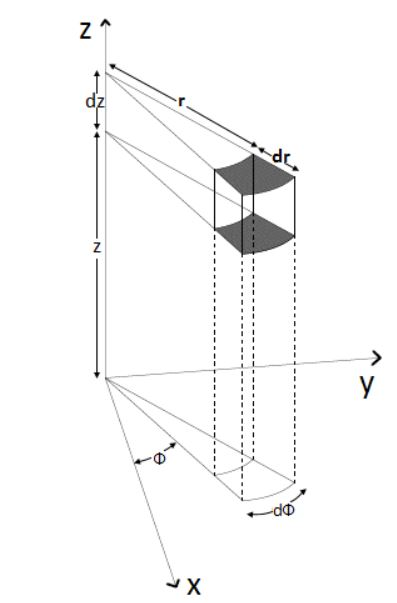
\includegraphics[width=0.2\linewidth]{EDPheat.JPG}
\end{center}
suponemos que tenemos una barra cilíndrica la cual tiene cierta distribución de calor que queremos conocer su cambio en un instante dado, por lo que análogo al análisis en coordenadas cartesianas, realizamos el balance de energía
\end{block}
    
\end{frame}

\begin{frame}{}

\begin{block}{}
\begin{center}
    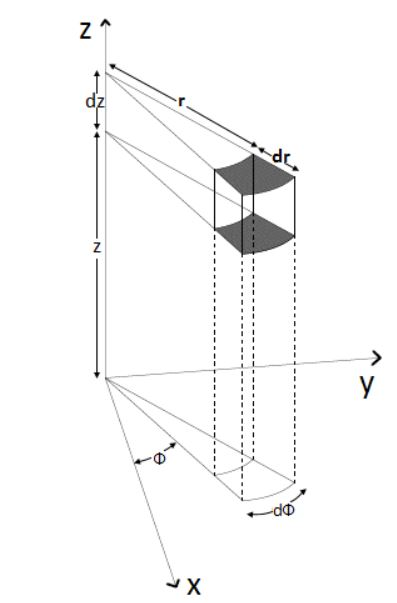
\includegraphics[width=0.2\linewidth]{EDPheat.JPG}
\end{center}
$$E_{st}=E_{in}-E_{out}+E_{gen},$$
en donde: 
\begin{itemize}
    \item $E_{st}:=$ Tasa a la que se almacena la energía térmica dentro de un volumen.
    \item $E_{in}:=$ Tasa a la que la energía entra.
    \item $E_{out}:=$ Tasa a la que la energía sale.
    \item $E_{gen}:=$ Tasa en la que se genera la energía dentro de la barra.
\end{itemize}
\end{block}

\end{frame}

\begin{frame}{}

\begin{block}{}
\begin{center}
    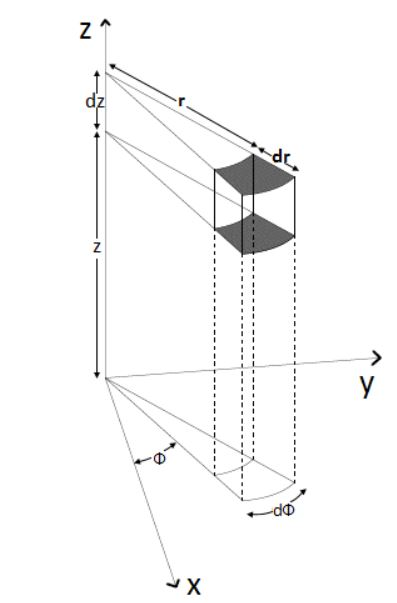
\includegraphics[width=0.2\linewidth]{EDPheat.JPG}
\end{center}
$$E_{in} = q_r + q_z + q_{\phi}$$
$$E_{out} = q_{r + dr} + q_{z + dz} + q_{\phi + d \phi}$$
Dimensionalmente en coordenadas cilíndricas $q_r$, $q_{z}$ y $q_{\phi}$, representan la energía que entra desde cada una de los lugares correspondientes de la sección del cilindro, si la energía entra desde el lugar $r$, en algún lugar $dr$ 'sale' la energía del sistema. Y de manera análoga ocurre con los otros dos componentes.
\end{block}

\end{frame}

\begin{frame}{}

\begin{block}{}
	\begin{center}
		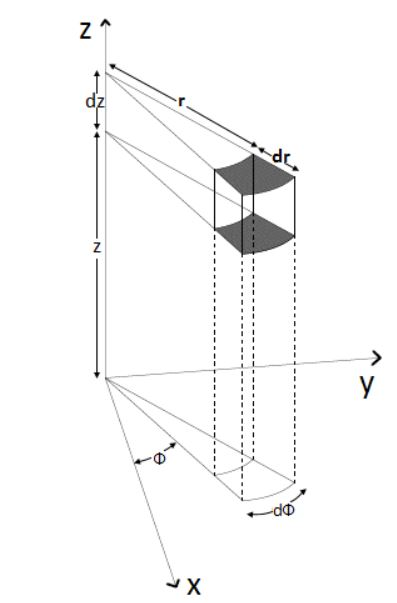
\includegraphics[width=0.2\linewidth]{EDPheat.JPG}
	\end{center}
	$$E_{gen} = \dot{q} \times \text{Volúmen} = \dot{q}(dr \cdot dz \cdot r  \cdot d\phi),$$
	en donde $\dot{q}$ representa un coeficiente de generación de energía y el volúmen, que como vemos es el producto entre los componentes diferenciales que utilizamos para definir nuestra sección.
\end{block}

\end{frame}

\begin{frame}{}

\begin{block}{}
	\begin{center}
		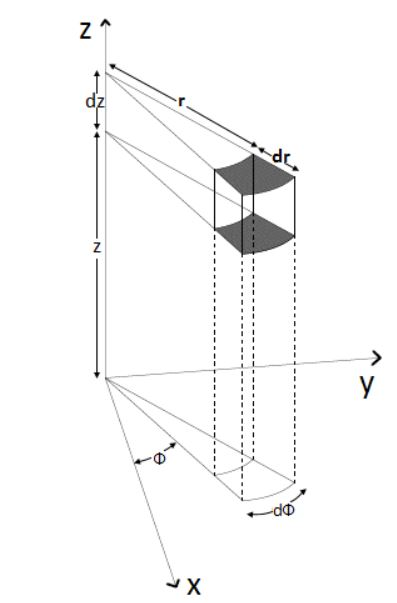
\includegraphics[width=0.2\linewidth]{EDPheat.JPG}
	\end{center}
	$$E_{st} = \rho (dr \cdot r \cdot d\phi \cdot dz) C_p \frac{dT}{dt},$$
	en donde $\dot{q}$ representa un coeficiente de generación de energía y el volúmen, que como vemos es el producto entre los componentes diferenciales que utilizamos para definir nuestra sección.
\end{block}

\end{frame}

\begin{frame}{}

\begin{block}{}
	Reemplazando los resultados anteriores tenemos:
	\begin{equation}
		\begin{split}
		\rho (dr \cdot r \cdot d\phi \cdot dz) C_p \frac{dT}{dt} = & (q_r + q_z + q_{\phi}) - (q_{r + dr} + q_{z + dz} + q_{\phi + d \phi}) \\
		&+ \dot{q}(dr \cdot dz \cdot r  \cdot d\phi))
		\end{split}
		\label{eq:heat_big}
	\end{equation}
ahora debemos analizar como 'sale' el calor respecto a como entra, para ello realizaremos la expansión series de Taylor, para $q_{r + dr}$ tendríamos:
$$q_{r + dr} = q_r + \frac{\partial q_r}{\partial r} dr,$$
y de la misma manera para los otros dos componentes:
$$q_{\phi + d\phi} = q_{\phi} + \frac{\partial q_{\phi}}{\partial \phi} d\phi, \text{  } q_{z + dz} = q_{z} + \frac{\partial q_{z}}{\partial z} dz,$$
Ahora reemplazando estos resultados en (\ref{eq:heat_big})
 
\end{block}

\end{frame}

\begin{frame}{}
Realizando la sustitución, tenemos
\begin{block}{}
	\begin{equation*}
	\begin{split}
	\rho (dr \cdot r \cdot d\phi \cdot dz) C_p \frac{dT}{dt} = & (q_r + q_z + q_{\phi}) - q_r - \frac{\partial q_r}{\partial r} dr \\
	&- q_{z} - \frac{\partial q_{z}}{\partial z} dz - q_{\phi} - \frac{\partial q_{\phi}}{\partial \phi} d\phi \\
	&+ \dot{q}(dr \cdot dz \cdot r  \cdot d\phi)),
	\end{split}
	\end{equation*}
	y simplificando,
	\begin{equation}
	\begin{split}
	\rho (dr \cdot r \cdot d\phi \cdot dz) C_p \frac{dT}{dt} &= - \frac{\partial q_r}{\partial r} dr - \frac{\partial q_{z}}{\partial z} dz - \frac{\partial q_{\phi}}{\partial \phi} d\phi \\
	&+ \dot{q}(dr \cdot dz \cdot r  \cdot d\phi)),
	\end{split}
	\label{eq:heat_big_2}
	\end{equation}
\end{block}

\end{frame}

\begin{frame}{}

\begin{block}{}
	Haciendo uso de la ley de calor de Fourier, tenemos que para $q_r$
	$$q_r = -k \frac{\partial T}{\partial r} r \cdot dz \cdot d\phi,$$
	en dónde $-k \frac{\partial T}{\partial r}$ representan el flujo térmico y $r \cdot dz \cdot d\phi$, el área de interés y nuevamente de manera análoga para los otros dos componentes, tenemos:
	$$q_z = -k \frac{\partial T}{\partial z} r \cdot dr \cdot d\phi, \text{   } q_\phi = -\frac{k}{r} \frac{\partial T}{\partial \phi} \cdot dr \cdot d\phi$$
\end{block}

\end{frame}

\begin{frame}{}

\begin{block}{}
	Sustituyendo los resultados anteriores en la ecuación (\ref*{eq:heat_big_2}),
	\begin{equation*}
	\begin{split}
	\rho (dr \cdot r \cdot d\phi \cdot dz) C_p \frac{dT}{dt} &= \frac{\partial}{\partial r} \left(kr\frac{\partial T}{\partial r}\right) d\phi \cdot dr \cdot dz\\
	&+ \frac{\partial}{\partial \phi} \left(\frac{k}{r}\frac{\partial T}{\partial \phi}\right) d\phi \cdot dr \cdot dz\\
	&+\frac{\partial}{\partial z} \left(k\frac{\partial T}{\partial z}\right) r \cdot d\phi \cdot dr \cdot dz\\
	&+\dot{q}(dr \cdot dz \cdot r  \cdot d\phi)
	\end{split}
	\end{equation*}
	Simplificando,
	\begin{equation}
	\rho C_p \frac{dT}{dt} = \frac{1}{r}\frac{\partial}{\partial r} \left(kr\frac{\partial T}{\partial r}\right) + \frac{1}{r^2}\frac{\partial}{\partial \phi} \left(\frac{k}{r}\frac{\partial T}{\partial \phi}\right) + \frac{\partial}{\partial z} \left(k\frac{\partial T}{\partial z}\right) + \dot{q}
	\end{equation}
	Que finalmente es la ecuación de calor en coordenadas cilíndricas.
\end{block}

\end{frame}

\end{document}